\documentclass[memoire.tex]{subfiles}

\chapter{Concepts formels}

\section{Introduction}
L'objectif de ce chapitre est dans un premier temps de rappeler des notions de probabilités~\cite{probaBio, decision_tree, apprentissage} qui serviront à la compréhension de ce document. Il s'agit ensuite d'expliquer dans sa généralité les concepts d'arbres décisionnels afin d'introduire des principes de classement et d'optimisation.

\section{Rappels de probabilité}
	\subsection{Expérience aléatoire}
Une expérience est dire aléatoire si les résultats possibles sont connus à l'avance sans vraiment savoir celui obtenu au préalable. On appelle univers, noté \(\Omega\), l'ensemble de toutes les issues possibles d'une expérience et \(\omega\) une réalisation de l'expérience.
\begin{equation}
\Omega = \begin{Bmatrix} \omega_1, \omega_2, \cdots, \omega_n \end{Bmatrix}, n \in \mathbb{N}
\end{equation}
		\subsection{Événements}
Un événement correspond à un ensemble de résultats possibles pour une expérience. Si cet ensemble est constitué d'un seul élément, on parle alors d'événement élémentaire. Si l'ensemble de résultats est égal à l'univers \(\Omega\), alors l'événement est dit certain. En revanche, si aucun résultat n'est présent (ensemble \(\emptyset\)), alors c'est un événement impossible.
		\subsection{Probabilités}
Une probabilité est une fonction qui à un événement A, associe un poids.
\begin{equation}
\left \{
\begin{array}{l}
P(\Omega) = 1 \\
P(\emptyset) = 0 \\
0 \leq P(A) \leq 1 \\
P(\bigcup_{i=1}^n A_i) = \sum_{i=1}^n P(A_i)
\end{array}
\right . 
\end{equation}
Plus la probabilité est proche de 1, plus il est possible que l'événement se réalise.
Soit A et B deux événements quelconques, \(P(A)\) est dite conditionnelle si son résultat est influencé par l'événement B :
\begin{equation} 
\left \{
\begin{array}{l}
B \neq \emptyset \\
P(B) \neq 0 \\
A = (A \cap B) \cup (A \cap \overline{B}) \\
\end{array}
\right . 
\end{equation}
On peut alors déduire deux formules : le théorème de Bayes (1.4) permettant de calculer \(P_B(A)\) et le théorème es probabilités totales (1.5) qui permet de connaitre la valeur de \(P(A)\) à partir de deux événements A et B. 
\begin{equation}
P_B(A) = \frac{P(A \cap B)}{P(B)}
\end{equation}
\begin{equation}
P(A) = P_B(A)P(B) + P_{\overline{B}}(A)P(\overline{B})
\end{equation}

\section{Arbre de décision}
\subsection{Définition}
Un arbre de décision est une représentation structurelle qui permet d'aboutir à un choix. C'est un graphe acyclique orienté composé :
\begin{itemize}
\item d'un sommet sans parents appelé racine,
\item de sommets appelés nœuds, correspondant à des tests,
\item de sommets terminaux nommés feuilles,
\item des arrêtes, ou branches, désignant chacune les résultats d'un test
\end{itemize}
Pour construire un arbre de décision, une approche \textit{Top-Down} est utilisée, appelée \textit{Top Down Induction of Decision Tree} (\textit{TDIDT}). Elle peut se décomposer en plusieurs parties :
\begin{enumerate}
\item Partir du jeu complet de données et construire la racine.
\item Réaliser un test afin de séparer les données.
\item Séparer le nœud actuel en fonction des résultats possibles.
\item Appliquer récursivement jusqu'à atteindre les feuilles.
\end{enumerate}
Lorsque chaque nœuds sont composés exactement de deux descendants (hors feuilles), on parle alors d'arbre de décision binaire. C'est un cas très largement utilisé des algorithmes de construction d'arbres tels que CART~\cite{ant_colony}, qui sera expliqué ultérieurement.
\subsection{Exemple}
Prenons comme exemple les données météorologiques présente dans la table 1. Cette table est constitué de différentes colonnes concernant différentes information ainsi qu'une colonne indiquant si la décision de sortir a été prise ou non. Dans un peu premier temps, il est possible de déduire les tests à réaliser comme par exemple "La température est-elle élevée ?" ou encore "Quel est le temps ?". A ces questions découlent des réponses possibles, \{oui, non\} pour la première et \{soleil, nuageux, pluie\} pour la deuxième. Une fois l'approche \textit{TDIDT} utilisée, un arbre de décision est alors obtenu (figure 1.1).

\begin{table}[!h]
\footnotesize
\centering
\renewcommand{\arraystretch}{2}
\begin{tabular}{|c|c|c|c|c|c|}
\hline
% thead
Jour &
Temps & 
Température & 
Humidité & 
Vent & 
Sortie\\
\hline
1  & soleil  	& élevée	& haute  	& faible 	& N \\
2  & soleil  	& élevée  	& haute   	& fort 		& N \\
3  & nuageux  	& élevée 	& haute   	& faible 	& Y \\
4  & pluie  	& moyenne   & haute 	& faible 	& Y \\
5  & pluie  	& basse 	& normale 	& faible 	& Y \\
6  & pluie		& basse		& normale   & fort 		& N \\
7  & nuageux	& basse   	& normale 	& fort 		& Y \\
8  & soleil 	& moyenne 	& haute   	& faible 	& N \\
9  & soleil 	& basse  	& normale	& faibles 	& Y \\
10 & pluie   	& moyenne 	& normale   & faible 	& Y \\
11 & soleil  	& moyenne   & normale 	& fort	 	& Y \\
12 & nuageux  	& moyenne   & haute 	& fort		& Y \\
13 & nuageux   	& élevée 	& normale 	& faible 	& Y \\
14 & pluie  	& moyenne	& haute   	& fort		& N \\
\hline
\end{tabular}
\caption{Table Météo}
\end{table}

\begin{figure}[!h]
	\centering
	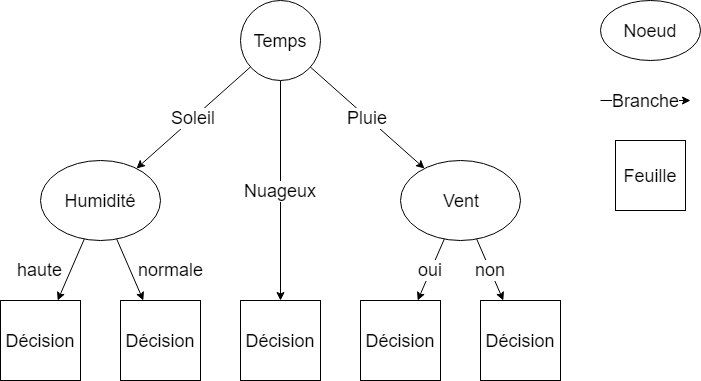
\includegraphics[scale=0.6]{img/decision_tree_meteo.png}
	\caption{Arbre de décision de la table Météo}
\end{figure}

\section{Arbre de décision pour le classement}
		\subsection{Attributs et classes}
Soit un ensemble d'observation \(S\) de taille \(n\):
\begin{equation}
S = \{s_1, s_2, ..., s_n\}.
\end{equation}
Chaque observation \(s_i\) est composée d'un ensemble de \(m\) attributs :
\begin{equation}
A_s = \{a_1, a_2, ..., a_m\}.
\end{equation}
Soit \(V_j\) l'ensemble de taille \(l\) des valeurs possibles de l'attribut \(a_j\) d'une observation \(s_i\) tels que :
\begin{equation}
V_j = \{ v_1, v_2, ..., v_l \}.
\end{equation}
La valeur de l'attribut \(a_j\) sera représentée par \(v_k\).
Un attribut est dit qualitatif si l'ensemble des valeurs possibles est symbolique (non numérique), par exemple si \(V_j\) représente les couleurs d'écriture d'un mot. On obtiendrait alors \( V_j = \{\) bleu, rouge, noir, vert \(\} \).\\

Une donnée est quantitative si l'ensemble des valeurs possibles est un ensemble numérique fini ou infini :
\begin{itemize}
\item Si un attribut peut prendre une infinité de valeurs dans son ensemble, alors celui-ci est qualifié de continu, par exemple le temps d'exécution d'un processus.
\item Dans le cas contraire, une variable dite discrète possède une valeur finie. Elle est généralement liée à une énumération, comme par exemple le nombre de trait dans un caractère. 
\end{itemize}

\(a_j\) est nominal si la notion d'ordre n'est pas présente dans l'ensemble des valeurs possibles, par exemple si \(V_j = \{\) un, deux, trois, quatre, cinq, six, sept, huit, neuf \(\} \) représente le nom d'un chiffre en toutes lettres.\\

Un attribut est ordinal si la notion les valeurs possibles contiennent la notion d'ordre. Cela peut être par exemple l'appréciation d'un client : \(V_j = \{\) mauvais, bon, très bon \(\} \)\\

Une variable est qualifiée de binaire si l'ensemble \(V_j\) des valeurs possibles est de taille \(l=2\)\\

La classe d'une observation correspond a une "catégorie" et permet de se rapprocher ou de se différencier des autres observations. Elle correspond à une feuille dans un arbre décisionnel.\\

Reprenons la table 1.1 (Météo), l'attribut jour correspond à l'identifiant dans l'observation et donc n'est pas pris en compte. \textit{Temps}, \textit{Température}, \textit{Humidité} et \textit{Vent} sont des attributs qualitatifs dont deux d'entre eux binaires : \(V_{Humidite} = \{haute, normale\}\) et \(V_{Vent} = \{fort, faible\} \). Chaque observation possède une classe \textit{Sortie} pouvant prendre Y ou N comme valeur.
		\subsection{Apprentissage supervisé}
Le domaine de l'apprentissage peut se séparer en deux types : le supervisé et le non-supervisé. \\

Dans le cas de l'apprentissage non-supervisé, le but recherché est d'assembler les similitudes entre les observations. Une des méthodes les plus communes est le \textit{clustering}~\cite{data_mining}.\\

Le second type d'apprentissage est dit supervisé. Dans ce cas, le but est d'apprendre du modèle pour arriver à déterminer la classe de l'observation. C'est dans ce domaine que se situe les arbres de décision. Les jeux de données sont alors séparés en deux : une partie jeu d'entrainement (\textit{training set}) et une partie jeu de test (\textit{test set}). Le but est d'apprendre du jeu d'entrainement afin de classer les observations du jeu de test. Soit C un ensemble de classe de taille n :
\begin{equation}
C = \{c_1, \cdots, c_n\}
\end{equation}
Classer une observation \(s_i\) revient à trouver le \(c_j\) qui lui correspond le mieux par le biais d'une fonction de classement F, calculé grâce au jeu de données d'entrainement.
		\subsection{Quantification de l'information}
La quantification de l'information permet de dégager une composante importante des tests d'un arbre de décision : le manque d'information. \textit{Dans la théorie de l'information, les notions de quantité d'information et d'incertitude sont équivalentes}~\cite{decision_tree, information_theory}. Partant de ces concepts, la quantité d'information h(x) d'une probabilité P(x) est une fonction croissante : si P(x) augmente, h(x) augmente. Par ailleurs, les événements certains et impossibles n'apportent aucune information étant donné que le résultat est connu d'avance.\\

Afin de mesurer le gain d'information, il est nécessaire d'introduire le concept d'entropie correspondant à l'impureté d'une observation en théorie de l'information~\cite{theory_communication}. Soit \(S\) un ensemble d'observations de taille \(n\) où \(s_i = \{\text{Y}, \text{N}\}\). L'entropie \(E\) de \(S\), où \(p_Y\) correspond à la probabilité d'avoir \(Y\) et \(p_N\) d'avoir \(N\)~\cite{machine_learning}, est définie par \begin{equation}
E(S) = - p_{Y}log_2p_{Y} - p_{N}log_2p_{N}
\end{equation}
La figure 1.2 représente la fonction d'entropie de S en fonction de $p_Y$. On observe que l'entropie est comprise entre 0 et 1 et vaut 0 lorsque $p_Y$ vaut 0 ou 1. Cela confirme le fait que les événements impossibles et certains n'apportent aucun gain d'information.\\

Nous venons de montrer l'entropie de S pour un attribut binaire. Par extension, si une observation $s_i$ peut prendre $l$ valeurs, alors 
\begin{equation}
E(S) = \sum_{i=1}^{l} - p_ilog_2p_i
\end{equation}

\begin{figure}[!h]  
\center
\begin{tikzpicture}
\begin{axis}[
    axis lines = left,
    xlabel = $p_t$,
    ylabel = {$E(S)$},
]
\addplot [
    domain=0:1, 
    samples=100, 
    color=black,
]
{-x*log2(x) - (1-x)*log2(1-x) };
\end{axis}
\end{tikzpicture}
\caption{Entropie de S en fonction de $p_t$}
\end{figure}
Par exemple, d'après la table 1.1, l'entropie de l'attribut sortie est égale à 
\begin{equation}
\begin{split}
E(Sortie) & = -\frac{9}{14}log_2(\frac{9}{14}) - \frac{5}{14}log_2(\frac{5}{14})\\
		  & = 0.4098 + 0.5305\\
		  & = 0.940
\end{split}
\end{equation}

GAIN
ARBRE METEO

\section{Arbre de décision pour l'optimisation}
quand arrêter un arbre
elagage
optimisation d'algorithmes (boosted etc)